\documentclass[12pt]{article}

\usepackage[margin=1in]{geometry}
\usepackage{amsmath,amsthm,amssymb}
\usepackage{tikz} % for drawing stuff
\usepackage{xcolor} % for \textcolor{}
\usepackage{readarray} % for \getargsC{}
\usepackage{graphicx} % disjoint union
\usepackage[utf8]{inputenc}
\usepackage[T1]{fontenc}
\usepackage{hyperref}


% Math sets
\newcommand{\N}{\mathbb{N}}
\newcommand{\Z}{\mathbb{Z}}
\newcommand{\R}{\mathbb{R}}

% Setup of project
\newenvironment{question}[2][Question]{\begin{trivlist}
\item[\hskip \labelsep {\bfseries #1}\hskip \labelsep {\bfseries #2.}]}{\end{trivlist}}
\newenvironment{answer}[2][Answer]{\begin{trivlist}
\item[\hskip \labelsep {\bfseries #1}\hskip \labelsep {\bfseries #2:}]}{\end{trivlist}}
\begin{document}
% math enumerate
\renewcommand{\theenumi}{\roman{enumi}}

% Short hands
\let\oldsum\sum
\renewcommand{\sum}[3]{\oldsum\limits_{#1}^{#2}#3}
\let\oldprod\prod
\renewcommand{\prod}[3]{\oldprod\limits_{#1}^{#2}#3}


\title{Homework 2}
\author{Haukur Páll Jónsson\\
NLP 2017}

\maketitle

\begin{question}{1}
Chomsky Normal Form (CNF)
\end{question}
\begin{answer}{a)}{}

The converted grammar is:
\begin{align*}
&S \to NP \text{  } VP \\
&S \to I\_VP \text{  } PP. \text{ We make the rule binary}\\
&I\_VP \to I \text{  } VP \\
&I \to i. \text{ When we make terminal symbols we do not make non-terminal symbols}\\
&NP \to Det \text{  } N\\
&VP \to V \text{  } NP. \text{ We use the fact that }V \to ate \text{ instead of creating a new rule which does exactly the same}\\
&VP \to ate. \text{ We eliminate unit rules}\\
&PP \to Pre \text{  } NP\\
&V \to ate\\
&Det \to the \text{ | }a\\
&N \to fork \text{ | }salad\\
&Pre \to with\\
\end{align*}
\end{answer}

\begin{question}{2}
PCFGs and the CYK algorithm
\end{question}

\begin{answer}{a)}

For any given parse, we compute the probability of that parse by; $p(rule)*p(element\, of \, rule)*p(element \, of \, rule)$
Lets start with the cell marked B: \\
$VP \to V \, Obj \, Obj$, we get: 0.3*0.6*0.2*0.2=0.0072 \\
$VP \to V \, Obj$, we get: 0.5*0.6*0.2=0.06 \\
$VP \to V \, small$, we get: 0.2*0.6*0.08=0.0096 \\
As we have three rules representing $VP$ we select the one which has the highest probability as the representatitve, namely $VP \to V \, Obj$.

For the cell marked A we essentially get the probabilities of B times 0.3: \\
%($S \to Subj \, VP$, we get: 1.0*0.3*0.0072=0,00216) \\
$S \to Subj \, VP$, we get: 1.0*0.3*0.06=0,018 \\
%($S \to Subj \, VP$, we get: 1.0*0.3*0.0096=0.00288) \\

% \begin{table}[]
% \centering
% \caption{My caption}
% \label{my-label}
% \begin{tabular}{|l|l|l|l|l|}
% \hline
%     & I                 & make              & her                                                                                    & duck                                                                                                                                                                                                              \\ \hline
% I    & $Subj \to I$, 0.3 & -                 & \begin{tabular}[c]{@{}l@{}}$S \to Subj VP$,\\   1.0*0.3*0.06\end{tabular}              & \begin{tabular}[c]{@{}l@{}}$S \to Subj VP$,\\   1.0*0.3*0.0072=0,00216\\ $S \to Subj VP$,\\   1.0*0.3*0.06=0,018\\ $S \to Subj VP$,\\   1.0*0.3*0.0096=0.00288\end{tabular}                                   \\ \hline
% make &                   & $V \to make$, 0.6 & \begin{tabular}[c]{@{}l@{}}$VP \to V \medskip Obj$, \\   0.5*0.6*0.2=0.06\end{tabular} & \begin{tabular}[c]{@{}l@{}}$VP \ to V Obj Obj$, \\   0.3*0.6*0.2*0.2=0.0072\\ $VP \to V Obj$,\\   0.5*0.6*0.2=0.06\\ $VP \to V small$,\\   0.2*0.6*0.08=0.0096\end{tabular}                                 \\ \hline
% her  &                   &                   & \begin{tabular}[c]{@{}l@{}}$Obj \to her$, 0.2\\ $Det \to her$, 1.0\end{tabular}        & \begin{tabular}[c]{@{}l@{}}$small \to Obj \medskip V$, \\   1.0*0.2*0.4=0.08\\ $NP \to Det \medskip N$, \\   0.5*1.0*0.5=0.25\\ $Subj \to NP$, \\   0.7*0.25=0.175\\ $Obj \to NP$, \\   0.8*0.25=0.2\end{tabular} \\ \hline
% duck &                   &                   &                                                                                        & \begin{tabular}[c]{@{}l@{}}$V \to duck$, 0.4\\ $N \to duck$, 0.5\\ $NP \to N$, 0.5*0.5=0.25\\ $Subj \to NP$, 0.7*0.25=0.175\\ $Obj \to NP$, 0.8*0.25=0.2\end{tabular}                                             \\ \hline
% \end{tabular}
% \end{table}
\end{answer}
\begin{answer}{b)}

  The most probable parse:

  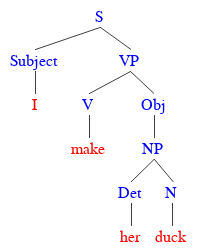
\includegraphics[scale=0.5]{tree}
  %In bracket notation the most probable parse is:
  %[S [Subject I] [VP [V make]  [Obj [NP [Det her] [N duck]] ]]]

\end{answer}

\begin{question}{3}
Dependency parsing /MST
\end{question}

\begin{answer}{a)}{CLE}

I denote each node as the first letter in the corresponding word, $John=j$, $likes=l$, $plain=p$ and $bagles=b$ and for the root, $root=r$. A directed edge from $i$ to $j$ is denoted by $(i,j)$. An edge with weight $k$ is denoted by $w((i,j))=k$.

After applying the first step of the algorithm we are left with the edges:\\
$E=\{(l,j),(p,l),(b,p),(l,b)\}$ \\
And corresonding weights: \\
$w((l,j))=20$, $w((p,l))=20$, $w((b,p))=15$, $w((l,b))=30$ \\
There is clearly three node a circle: $C=\{(p,l),(l,b),(b,p)\}$
\end{answer}

\begin{answer}{b)}{Final step}

The final result is: \\
$E=\{(r,l),(l,j),(l,b),(b,p)\}$ \\
And corresonding weights: \\
$w((r,l))=15$, $w((l,j))=20$, $w((l,b))=30$, $w((b,p))=15$ \\
Total span is 80.
\end{answer}

\begin{question}{4}
Dependency parsing / Transistion based
\end{question}

\begin{answer}{a)}{Arc-standard system}


\begin{table}[h!]
\centering
\caption{Configurations}
\label{my-label}
\begin{tabular}{|l|l|l|l|}
\hline
Transition       & Stack                       & Buffer                             & Arcs                                                                                                                                          \\ \hline
/                & {[}root{]}                  & {[}A koala eats leafs and barks{]} & $\emptyset=A$                                                                                                                                   \\ \hline
SHIFT            & {[}root A{]}                & {[}koala eats leafs and barks{]}   & $A$                                                                                                                                   \\ \hline
SHIFT            & {[}root A koala{]}          & {[}eats leafs and barks{]}         & $A$                                                                                                                                   \\ \hline
LEFT-ARC (det)   & {[}root koala{]}            & {[}eats leafs and barks{]}         & $A \cup\{koala \to A\}$                                                                                                                             \\ \hline
SHIFT            & {[}root koala eats{]}       & {[}leafs and barks{]}              & $A$                                                                                                                             \\ \hline
LEFT-ARC (nsubj) & {[}root eats{]}             & {[}leafs and barks{]}              & $A \cup\{eats \to koala\}$                                                                                                             \\ \hline
SHIFT            & {[}root eats leafs{]}       & {[}and barks{]}                    & $A$                                                                                                             \\ \hline
SHIFT            & {[}root eats leafs and{]}   & {[}barks{]}                        & $A$                                                                                                             \\ \hline
RIGHT-ARC (cc)   & {[}root eats leafs{]}       & {[}barks{]}                        & $A \cup\{leafs \to and\}$                                                                                              \\ \hline
SHIFT            & {[}root eats leafs barks{]} & {[}{]}                             & $A$                                                                                              \\ \hline
RIGHT-ARC (conj) & {[}root eats leafs{]}       & {[}{]}                             & $A \cup\{leafs \to barks\}$                            \\ \hline
RIGHT-ARC (dobj) & {[}root eats{]}             & {[}{]}                             & $A \cup\{eats \to leafs\}$              \\ \hline
RIGHT-ARC (root) & {[}root{]}                  & {[}{]}                             & $A \cup\{root \to eats\}$ \\ \hline
\end{tabular}
\end{table}
\end{answer}
\end{document}
